\ifsubmission
\begin{figure*}[t]
  \centering
  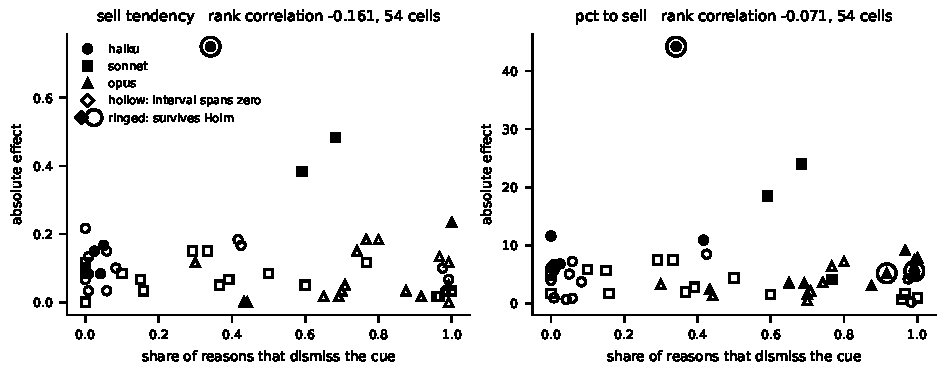
\includegraphics[width=\textwidth]{../figures/fig6_dissociation_acl.pdf}
  \caption{Dismissing the cue does not predict not acting on it. Each point
  is one model, effort and family cell: on the horizontal axis the share of
  that cell's one-sentence reasons that name the manipulated cue and discount
  it, on the vertical axis the size of that cell's effect, unsigned, because
  the claim is about magnitude. Only the six families the advisor ever refers
  to appear; the other three are never referred to at all, which the text
  takes up. If saying the right thing meant doing the right thing, the cloud
  would run downhill. The two Opus cells that survive Holm
  correction, at the right of the continuous panel, discount the cue in over
  nine tenths of their reasons and move with it anyway.}
  \label{fig:dissociation}
\end{figure*}
\else
\begin{figure}[t]
  \centering
  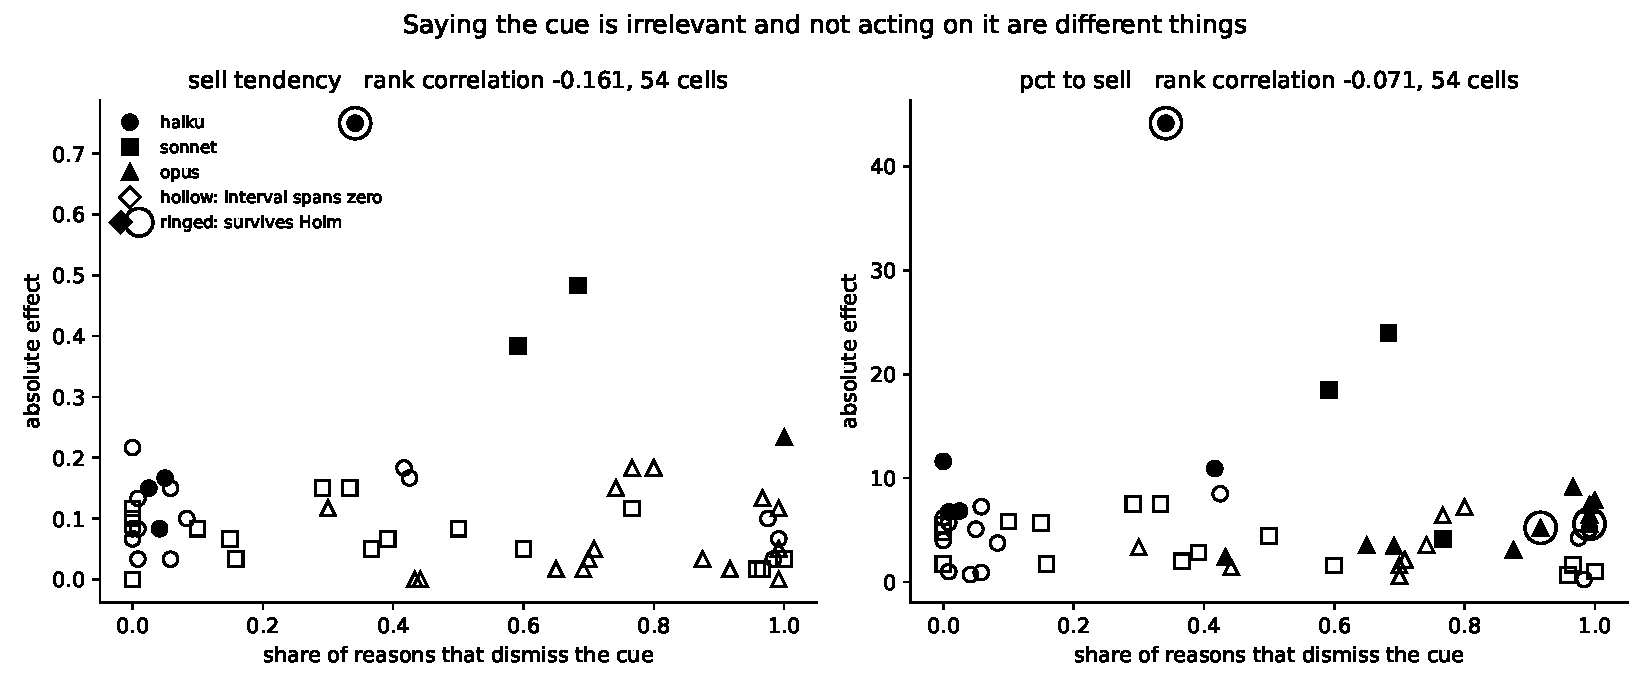
\includegraphics[width=\linewidth]{../figures/fig6_dissociation.pdf}
  \caption{Rejection rate against absolute effect, one point per model,
  effort and family cell, over the six families the advisor refers to. A flat
  cloud is the finding: the cells that discount the cue most are not the
  cells that move least.}
  \label{fig:dissociation}
\end{figure}
\fi
